\documentclass[11pt,a4paper]{article}
\usepackage{graphicx}
\usepackage{amssymb, amsmath}
\usepackage{url}
\usepackage{polski}
\usepackage{subfigure}
\usepackage[utf8]{inputenc} 

\title{Interpreter skryptów dla platformy Android OS\\ \large Dokumentacja końcowa}
\author{Piotr Jastrzębski\\ \url{piotr.jastrzebski@gmail.com}}
\date{}
\begin{document}
\maketitle

\section{Opis funkcjonalności}
Projekt funkcjonuje jako integralna część aplikacji, realizowanej na potrzeby pracy inżynierskiej, ale na potrzeby testów może korzystać z modułu funkcji kontrolnych, niezwiązanych z przetwarzaniem obrazu. Działa pod kontrolą systemu Android, a napisany został w Javie. W celu stworzenia zarówno leksera jak i parsera wykorzystałem możliwości programu ANTLR v3., który to na podstawie zadanej gramatyki generuje parser typu LL(*). W związku z koniecznością wielokrotnego testowania różnych funkcji aplikacji wektoryzacji obrazów bitmapowych z różnymi parametrami, interpreter zapewnia taką możliwość, bez konieczności każdorazowej kompilacji. Wielokrotne wywołania mogą zostać wywołane skryptem z zastosowaniem pętli do...while, a parametry wywołań mogą być zależne od zmiennych. Założeniem było stworzenie interpretera obsługującego wczytywanie skryptów wywołań z poziomu interfejsu graficznego aplikacji. Skrypt powinien zostać przygotowany zgodnie z opisem i uwzględnieniem przeznaczenia zmiennych i wywołań podanymi w punkcie \ref{zmienne}. Gramatyka wywołań została przedstawiona w punkcie \ref{gramatyka}.

\subsection{Specyfikacja formalna}\label{zmienne}
Plik skryptowy dla aplikacji powinien być zapisany w formacie tekstowym z zachowaniem rozszerzenia pliku {\tt "txt"}, np. {\tt "skrypt.txt"}. Obecność białych znaków nie wpływa na działanie aplikacji. Poprawny skrypt musi zawierać wczytanie obrazu wzorcowego i zapis do pliku wyniku w postaci wektorowej. Zmienne liczbowe oraz ścieżka zapisu mogą być zależne od wartości zmiennej iteratora. Wartości argumentów funkcji uzależnić można poprzez zastosowanie wyrażenia arytmetycznego (z wykorzystaniem operacji dodawania, odejmowania, mnożenia i dzielenia) mogącego wykorzystywać równocześnie wartości liczbowe oraz zmienne. Do ścieżki poprzez dodanie zmiennej w postaci {\tt +n+} przed rozszerzeniem pliku można uzależnić wczytywany lub zapisywany w projekcie plik. (przyjmując, że {\tt n} wybrano jako symbol zmiennej) Poniżej przedstawiono listę przeznaczenia poszczególnych zmiennych wszystkich funkcji skryptu.
\begin{verbatim}
load(
   path           //bezwzględna ścieżka obrazu
)

hough_c(
   dp,            //odwrócony współczynnik proporcjonalności
                  //akumulatora (I)
   minDist,       //minimalna odległość pomiędzy
                  //środkami okręgów (D)
   gaussSize,     //rozmiar maski filtra Gaussa (D)
   gaussSigma     //współczynnik sigma filtra Gaussa (D)
)

hough_l(
   rho,           //rozdzielczość akumulatora w pikselach (I)
   theta,         //rozdzielczość akumulatora w radianach (D)
   threshold,     //wartość progowa akumulatora (I)
   minLineLength, //minimalna długość odcinka (I)
   maxLineGap,    //maksymalna długość przerwy (I)
   cannyT1,       //mniejsza wartość progowa detektora Cannyego (I)
   cannyT2        //większa wartość progowa detektora Cannyego (I)
)

harris(
   maxCorners,    //maksymalna liczba zwracanych wierzchołków (I)
   qualityLevel,  //minimalna "jakość" wierzchołka (D)
   minDistance,   //minimalna odległość między zwracanymi
                  //wierzchołkami (I)
   blockSize,     //rozmiar sąsiedztwa (I)
   useHarris,     //korzysta z detektora Harrisa dla "true",
                  //dla "false" z cornerMinEigenVal() (D)
   k              //wolny parametr detektora Harrisa (D)
)

save(
   path           //bezwzględna ścieżka rezultatu
)

do
{...}             //funkcje w pętli
while(
   var            //zmienna lub wartość
   op             //relacja: <, >, <=, >=, ==, !=
   n              //zmienna lub wartość
)

var               //nazwa zmiennej
=
n                 //przypisywana wartość lub wyrażenie
              
var               //nazwa zmiennej (jedna litera)
op                //operator +=, -=, /=, *=
n                 //zmiana wartości zmiennej lub wyrażenie

progress          //znacznik postępu
\end{verbatim}

\section{Wymagania funkcjonalne}
\begin{itemize}
\item{parsowanie skryptów zapisanych w plikach tekstowych}
\item{umożliwienie wielokrotnego wykonywania wywołań zamkniętych w pętli do...while i zależnych od iteratora}
\item{przestrzeganie logicznego porządku wczytanie-funkcje-zapis}
\item{możliwość wywoływania funkcji wielokrotnie i w dowolnej kolejności}
\item{kontrola poprawności wprowadzonych danych}
\item{informowanie użytkownika, w którym miejscu skryptu wystąpił błąd}
\end{itemize}

\section{Wymagania niefunkcjonalne}
Projekt powstaje jako integralna część programu wektoryzacji obrazów bitmapowych realizowanego na potrzeby pracy inżynierskiej. Konieczne jest poszerzenie interfejsu użytkownika o dodatkowy przycisk wywołujący parsowanie skryptu. Ścieżkę do skryptu definiuje się w aktualnie istniejącym polu tekstowym aplikacji. Zrzuty ekranu z działania aplikacji przedstawiono na rysunku \ref{android}.

\section{Realizacja}
Aplikacja parsera składa się z kilku modułów: skanera, parsera i analizatora składniowego. Schemat przekazywania informacji pomiędzy modułami, a także między elementami parsera a aplikacją wektoryzującą przedstawiono na rysunku \ref{schemat}. Tablica symboli jest tablicą globalną i przy wystąpieniu w strukturze skryptu nowego symbolu umieszcza go w strukturze tablicy. Symbole te wykorzystywane są potem podczas generacji i wykonywania kodu.
\\Klasy programu:
\begin{itemize}
\item \emph{StartActivity:} 	klasa UI (obsługa zdarzeń przycisków, przechwytywanie ścieżki skryptu, komunikacja z użytkownikiem)
\item \emph{ScriptInterpreter:} klasa obsługi skryptów (obsługa plików, czytanie znaków ze strumienia)
\item \emph{SymbolTable:} klasa implementująca obsługę tablicy symboli
\item \emph{TkomLexer:} klasa skanera (rozbicie tekstu, pomijanie białych znaków, rozpoznawanie tokenów)
\item \emph{TkomParser:} klasa parsera (sprawdzanie zgodności z gramatyką)
\item \emph{TkomSemantic:} klasa analizatora składniowego (sprawdzanie zgodności semantycznej skryptu z założeniami)
\item \emph{Dummies:} klasa zapewniająca mapowanie funkcji skryptu na funkcje programu
\item \emph{ProcessImage:} klasa przetwarzania obrazu (wykonuje funkcje graficzne na obrazie, zapisuje plik SVG)
\end{itemize}
\begin{figure}
\centering
\mbox{
\subfigure[Skrypt niepoprawny]{
\includegraphics[width=0.45\textwidth]{skrypt.png}}\quad
\subfigure[Skrypt poprawny]{
\includegraphics[width=0.45\textwidth]{skrypt2.png} }
}
\caption{Wygląd okna aplikacji w systemie Android}\label{android} 
\end{figure}
\begin{figure}
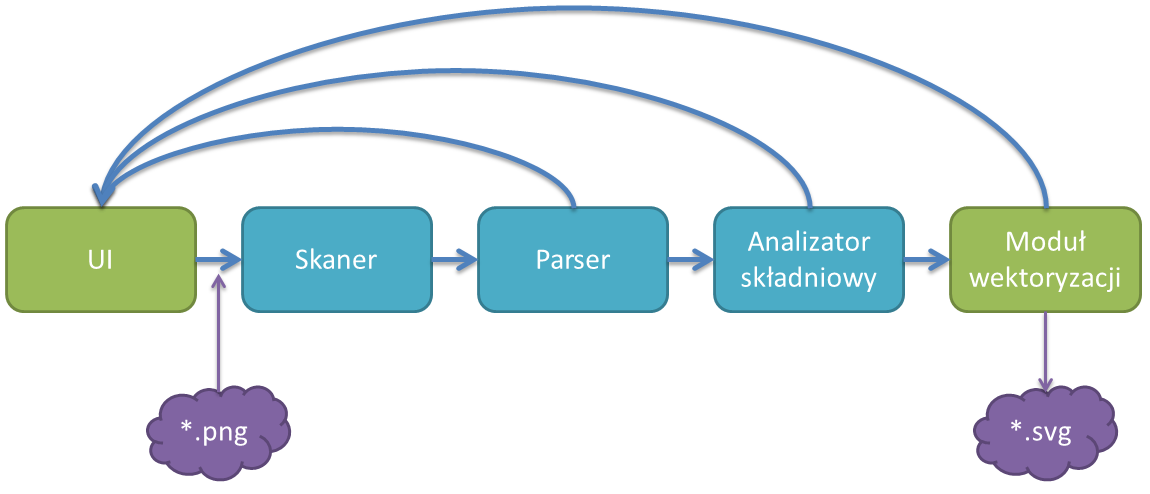
\includegraphics[width=\textwidth]{schemat.png}
\caption{Schemat zależności między modułami aplikacji.}
\label{schemat}
\end{figure}

\subsection{Analiza leksykalna (skanowanie)}
Polega na rozbiciu wczytanego z pliku tekstu na leksemy. Podczas skanowania ignorowane są wszelkie białe znaki. Następnie na podstawie leksemów zostają rozpoznane tokeny (odpowiednie przypasowanie do wzorca). Skaner rozpoznaje następujące tokeny:\\\\
\begin{tabular}{ | l | l | }
\hline                        
\bf{Przykład leksemu} & \bf{Token} \\\hline        
load & wyróżnik funkcji \\
save&\\
houghC&\\
houghL&\\
harris&\\
do&\\
\hline
progress& znacznik postępu\\\hline
( & początek funkcji\\\hline
) & koniec funkcji\\\hline
\{ & początek pętli \\\hline
\} & koniec pętli \\\hline
- & minus \\\hline
, & przecinek\\\hline
x & zmienna\\\hline
!= & operator\\\hline
123 & liczba naturalna\\\hline
1.23 & liczba dziesiętna\\\hline
"/mnt/sdacrd/bsc/a.jpg" & napis\\\hline
true & wartość logiczna\\\hline
\end{tabular}
\\\\\\
{\bf Gramatyka języka w notacji EBNF}\label{gramatyka}
Zmieniona względem wstępnej składni, nowa pozwala na tworzenie zmiennych o dowolnych nazwach, wykonywanie wyrażeń arytmetycznych zgodnie z priorytetami operatorów (zarówno w wywołaniach funkcji jako argumenty jak i poprzez globalne modyfikowanie wartości), konkatenacje stringów w przypadku ścieżki do pliku oraz implementuje pętle do...while z możliwością wielokrotnego zagnieżdżania.
\begin{verbatim}
MINUS	:	'-';
					
QUOTATION_MARK	:	'"';

ROUND_LEFT_BRACKET	:	'(';
	
ROUND_RIGHT_BRACKET	:	')';
	
CURLY_LEFT_BRACKET	:	'{';
	
CURLY_RIGHT_BRACKET	:	'}';
	
COMA	:	',';

EQUALS_SIGN	:	'=';	

EXTENSION_IN	:	'jpg' | 'jpeg' | 'bmp' | 'gif' | 'png'
              |'JPG' | 'JPEG' | 'BMP' | 'GIF' | 'PNG';
	
EXTENSION_OUT	:	'svg' | 'SVG';
	
LOAD	:	'load';

SAVE	:	'save';

ASS	:	'ass';

MOD	:	'mod';

HOUGHC	:	'houghC';

HOUGHL	:	'houghL';

HARRIS	:	'harris';

DO	:	'do';

WHILE	:	'while';

PROGRESS:	'progress';

VAR	:	('a'..'z'|'A'..'Z') ('a'..'z'|'A'..'Z'|'0'..'9'|'_')*;

REL	:	 '<' | '>' | '<=' | '>=' | '==' | '!=' ;

VARDEP	:	OPERATOR VAR;

OPERATOR	:	'-='|'+='|'*='|'/='	;
	
NUM	:	INT|DBL;

INT	:	('0'..'9')+;

DBL	:	(('0'..'9')+ '.' ('0'..'9')* EXPONENT?
    		|'.' ('0'..'9')+ EXPONENT?
    		|('0'..'9')+ EXPONENT);

EXPONENT:	('e'|'E') ('+'|'-')? ('0'..'9')+ ;

COMMENT	:	'//' ~('\n'|'\r')* '\r'? '\n'
    		|'/*' ( options {greedy=false;} : . )* '*/'
		;

WS	:	( ' '
        	| '\t'
        	| '\r'
        	| '\n'
        	) ;
\end{verbatim}
Dla przykładu:
\begin{verbatim}
load("/mnt/sdcard/bsc/1.jpg")
harris(99, 0.01, 58, 3, true, 0.04)
save("/mnt/sdcard/bsc/w1.svg")
\end{verbatim}
analiza leksykalna wyglądałaby tak:
\begin{center}
\begin{tabular}{ | l | l | l | }
\hline                        
\bf{Leksem} & \bf{Token} & \bf{Atrybut} \\ \hline        
load & wyróżnik funkcji & load\\ \hline
(& początek funkcji & \\ \hline    
"/mnt/sdcard/bsc/1.jpg" & napis & /mnt/sdcard/bsc/1.jpg\\ \hline   
) & koniec funkcji &\\ \hline   
harris & wyróżnik funkcji & harris\\ \hline
(& początek funkcji & \\ \hline  
99 & liczba naturalna &99\\ \hline   
, & przecinek &\\ \hline   
0.01 & liczba dziesiętna &0.01\\ \hline   
, & przecinek &\\ \hline    
58 & liczba naturalna &58\\ \hline   
, & przecinek &\\ \hline   
3 & liczba naturalna &3\\ \hline   
, & przecinek &\\ \hline   
true & wartość logiczna & true\\ \hline   
, & przecinek &\\ \hline   
0.04 & liczba dziesiętna &0.04\\ \hline   
) & koniec funkcji &\\ \hline   
save & wyróżnik funkcji & save\\ \hline
( & początek funkcji & \\ \hline
"/mnt/sdcard/bsc/w1.svg" & napis & /mnt/sdcard/bsc/w1.svg\\ \hline   
) & koniec funkcji &\\ \hline   
\end{tabular}
\end{center}

\subsection{Analiza składniowa (parsowanie)}
Analizator składniowy (parser) otrzymawszy od skanera ciąg symboli leksykalnych sprawdza czy może on zostać wygenerowany przez gramatykę. Tworzone jest drzewo składni na podstawie zapytania i sprawdzana są możliwości wykonania zapytania. W przypadku niemożliwości wygenerowania parser zgłasza błąd, o którym informuje użytkownika i przerywa interpretację.
\\\\
{\bf Lista produkcji:}
\begin{verbatim}

eval
	:	(load
		|save 
		|houghc
		|houghl 
		|harris
		|doWhileLoop 	
		|ass 		
		|mod 	
		|PROGRESS )+ ;
	
load	
	:	LOAD
		ROUND_LEFT_BRACKET
		QUOTATION_MARK
		path
		EXTENSION_IN 
		QUOTATION_MARK
		ROUND_RIGHT_BRACKET ;
		
save	
	: 	SAVE
		ROUND_LEFT_BRACKET
		QUOTATION_MARK
		path 
		EXTENSION_OUT
		QUOTATION_MARK
		ROUND_RIGHT_BRACKET ;	
		
path	
	:	(pathPart)+
		(
		'+'
		VAR
		'+'
		)?
		'.'	;

pathPart
	:	'/' ( VAR | INT )+ ;
		 
houghc
	:	HOUGHC
		ROUND_LEFT_BRACKET
		additionExp
		COMA
		additionExp 
		COMA
		additionExp 
		COMA
		additionExp 
		ROUND_RIGHT_BRACKET ;
		
houghl	
	:	HOUGHL
		ROUND_LEFT_BRACKET
		additionExp
		COMA
		additionExp
		COMA
		additionExp
		COMA
		additionExp
		COMA
		additionExp
		COMA
		additionExp
		COMA
		additionExp
		ROUND_RIGHT_BRACKET ;

harris	
	:	HARRIS
		ROUND_LEFT_BRACKET
		additionExp 
		COMA
		additionExp 
		COMA
		additionExp 
		COMA
		additionExp
		COMA
		logic_val 
		COMA
		additionExp 
		ROUND_RIGHT_BRACKET ;
		
doWhileLoop
	:	      
	    DO
	    CURLY_LEFT_BRACKET
		eval
	    CURLY_RIGHT_BRACKET
	    WHILE
		ROUND_LEFT_BRACKET
		additionExp 
		REL 
		additionExp 
		ROUND_RIGHT_BRACKET ;

ass	
	:	VAR 
		EQUALS_SIGN
		additionExp ;

mod
	:	VAR 
		OPERATOR
		additionExp	;
	
additionExp
	:	multiplyExp 
         	('-' multiplyExp
         	|'+' multiplyExp)* ;

multiplyExp 
	:	atomExp ('*' atomExp | '/' atomExp )* ;

atomExp
	:	(MINUS)?
		(NUM
		| VAR
		|'(' additionExp ')' );

logic_val 
	:	('TRUE' | 'true') | ('FALSE' | 'false');
\end{verbatim}

\subsection{Analiza semantyczna}
Po zakończeniu faz analizy leksykalnej i analizy składniowej następuje analiza semantyczna. Język skryptu obsługuje typowanie dynamiczne. O ile sama zmienna reprezentuje w ogólności dowolny typ, to w przypadku wywołania funkcji z argumentem nieodpowiedniego typu parser zwróci błąd. Tym samym, zadaniem tej fazy jest sprawdzenie programu źródłowego pod względem semantycznej zgodności z definicją języka źródłowego:
\begin{itemize}
\item kontrola zgodności wartości argumentów funkcji (typu całkowitego i podwójnej precyzji) z definicją
\item sprawdzanie, czy zmienna użyta w funkcji, została wcześniej zainicjalizowana
\item ewentualne rzutowanie
\end{itemize}
\section{Przykłady testowe}
\subsection{Pozytywne}
Powinny zrealizować wczytanie, zrealizowanie funkcji przetwarzania obrazów, a następnie zapisanie wyników wykrywania tych elementów w sposób wektorowy do pliku SVG:
\begin{itemize}

\item Wykrywanie okręgów, odcinków, wierzchołków.
\begin{verbatim}
load("/mnt/sdcard/bsc/1.jpg")
houghC(1.150, 58, 9, 2)
houghL(1, 0.0174532925, 10, 10, 10, 50, 200)
harris(99, 0.01, 58, 3, true, 0.04)
save("/mnt/sdcard/bsc/wynik_skrypt1.svg")
\end{verbatim}

\item Wykrywanie odcinków.
\begin{verbatim}
load("/mnt/sdcard/camera/DCIM1209.jpeg")
houghL(1, 0.02, 10, 5, 20, 75, 100)
save("/mnt/sdcard/test/test.svg")
\end{verbatim}
\end{itemize}
\subsection{Negatywne}
\begin{itemize}
\item Parser powinien zwrócić błąd dla:

\begin{verbatim}
load("/mnt/sdcard/bsc/1.jpg)     //brak domknięcia cudzysłowu
houghC(1.150, 58, 9)             //zbyt mała liczba argumentów
ass(xy, -12.3)                   //nieprawidłowa zmienna
xyz(99, 0.01, 58, 3, true, 0.04) //nieznana funkcja
save("/mnt/sdcard+x+/wynik.svg") //uzależnienie od zmiennej
                                 //w złym miejscu
\end{verbatim}
\end{itemize}
\end{document}
